\documentclass[../main]{subfiles}
\usepackage{lastpage,xr,refcount,etoolbox}
%\externaldocument{../Appendices/Appendix1-CodigosBase}
\begin{document}
\chapter{Training the Model}

{
\hypersetup{linkcolor=black}
\renewcommand{\contentsname}{Training the Model}
\minitoc % Muestra minitoc
}
In this chapter, we will demonstrate, through code and explanation, the steps needed to successfully train our YOLO model to recognize rock-paper-scissors gestures using the dataset prepared in the previous chapter. We will also cover how to utilize powerful NVIDIA GPUs in the cloud for free to meet the computational requirements of this process.

\section{Nvidia's GPUs to do our work}
To train a model of this scale, the power of our computer’s CPU is insufficient. Therefore, we use Google Colab for training the model with our generated dataset. Google Colab provides us with an Nvidia T4 GPU with 12GB of VRAM. Given that we plan to train the YOLOv8n.pt model, which has approximately 3 million parameters, this GPU will be adequate for the task. After creating the account and setting up the Jupyter notebook, we select the T4 GPU and execute the following command:
\begin{lstlisting}
!nvidia-smi
!pip install ultralytics
\end{lstlisting}
After that, we run the Python script we created to set up the folder structure. Next, we execute the Python script in our notebook that will be used to train our model:
\begin{lstlisting}
def train_model(yaml_file, epochs, project):
    model = YOLO(model="yolov8n.pt", task="detect")
    model.to('cuda')
    model.train(data = yaml_file,
        	  epochs = epochs,
              project = project,
        	  batch = 8,
              name = "train")          
    # batch = 8 is neccesary because GPU does not support higher

    results2 = model.val(data = yaml_file,
                        project = project,
                        batch = 8,
                        name = "test",
                        split = "test")

    # Create the full path for the text file
    metrics_file_path2 = os.path.join(project, "testing_metrics.txt")

    # Write the metricts in the text file
    with open(metrics_file_path2, 'w') as f:
        ...
\end{lstlisting}
Now, we set up the entire dataset structure, and immediately afterward, we train our model for the desired number of epochs (in my case, I will choose 32) and we wait for the results:
\begin{lstlisting}
prepare_structure()
train_model(f"{cd}/dataset_split/config.yaml", 32, "Hands_Tracking_Model")
\end{lstlisting}
\section{Model's training results}
Once the training process has finished (which took around 2 hours), we obtain a folder containing the trained model. Inside we can obtain plenty of information as well as results.png that contains the graphs with the different metrics of the output model:
\begin{figure}[H]
     \centering
     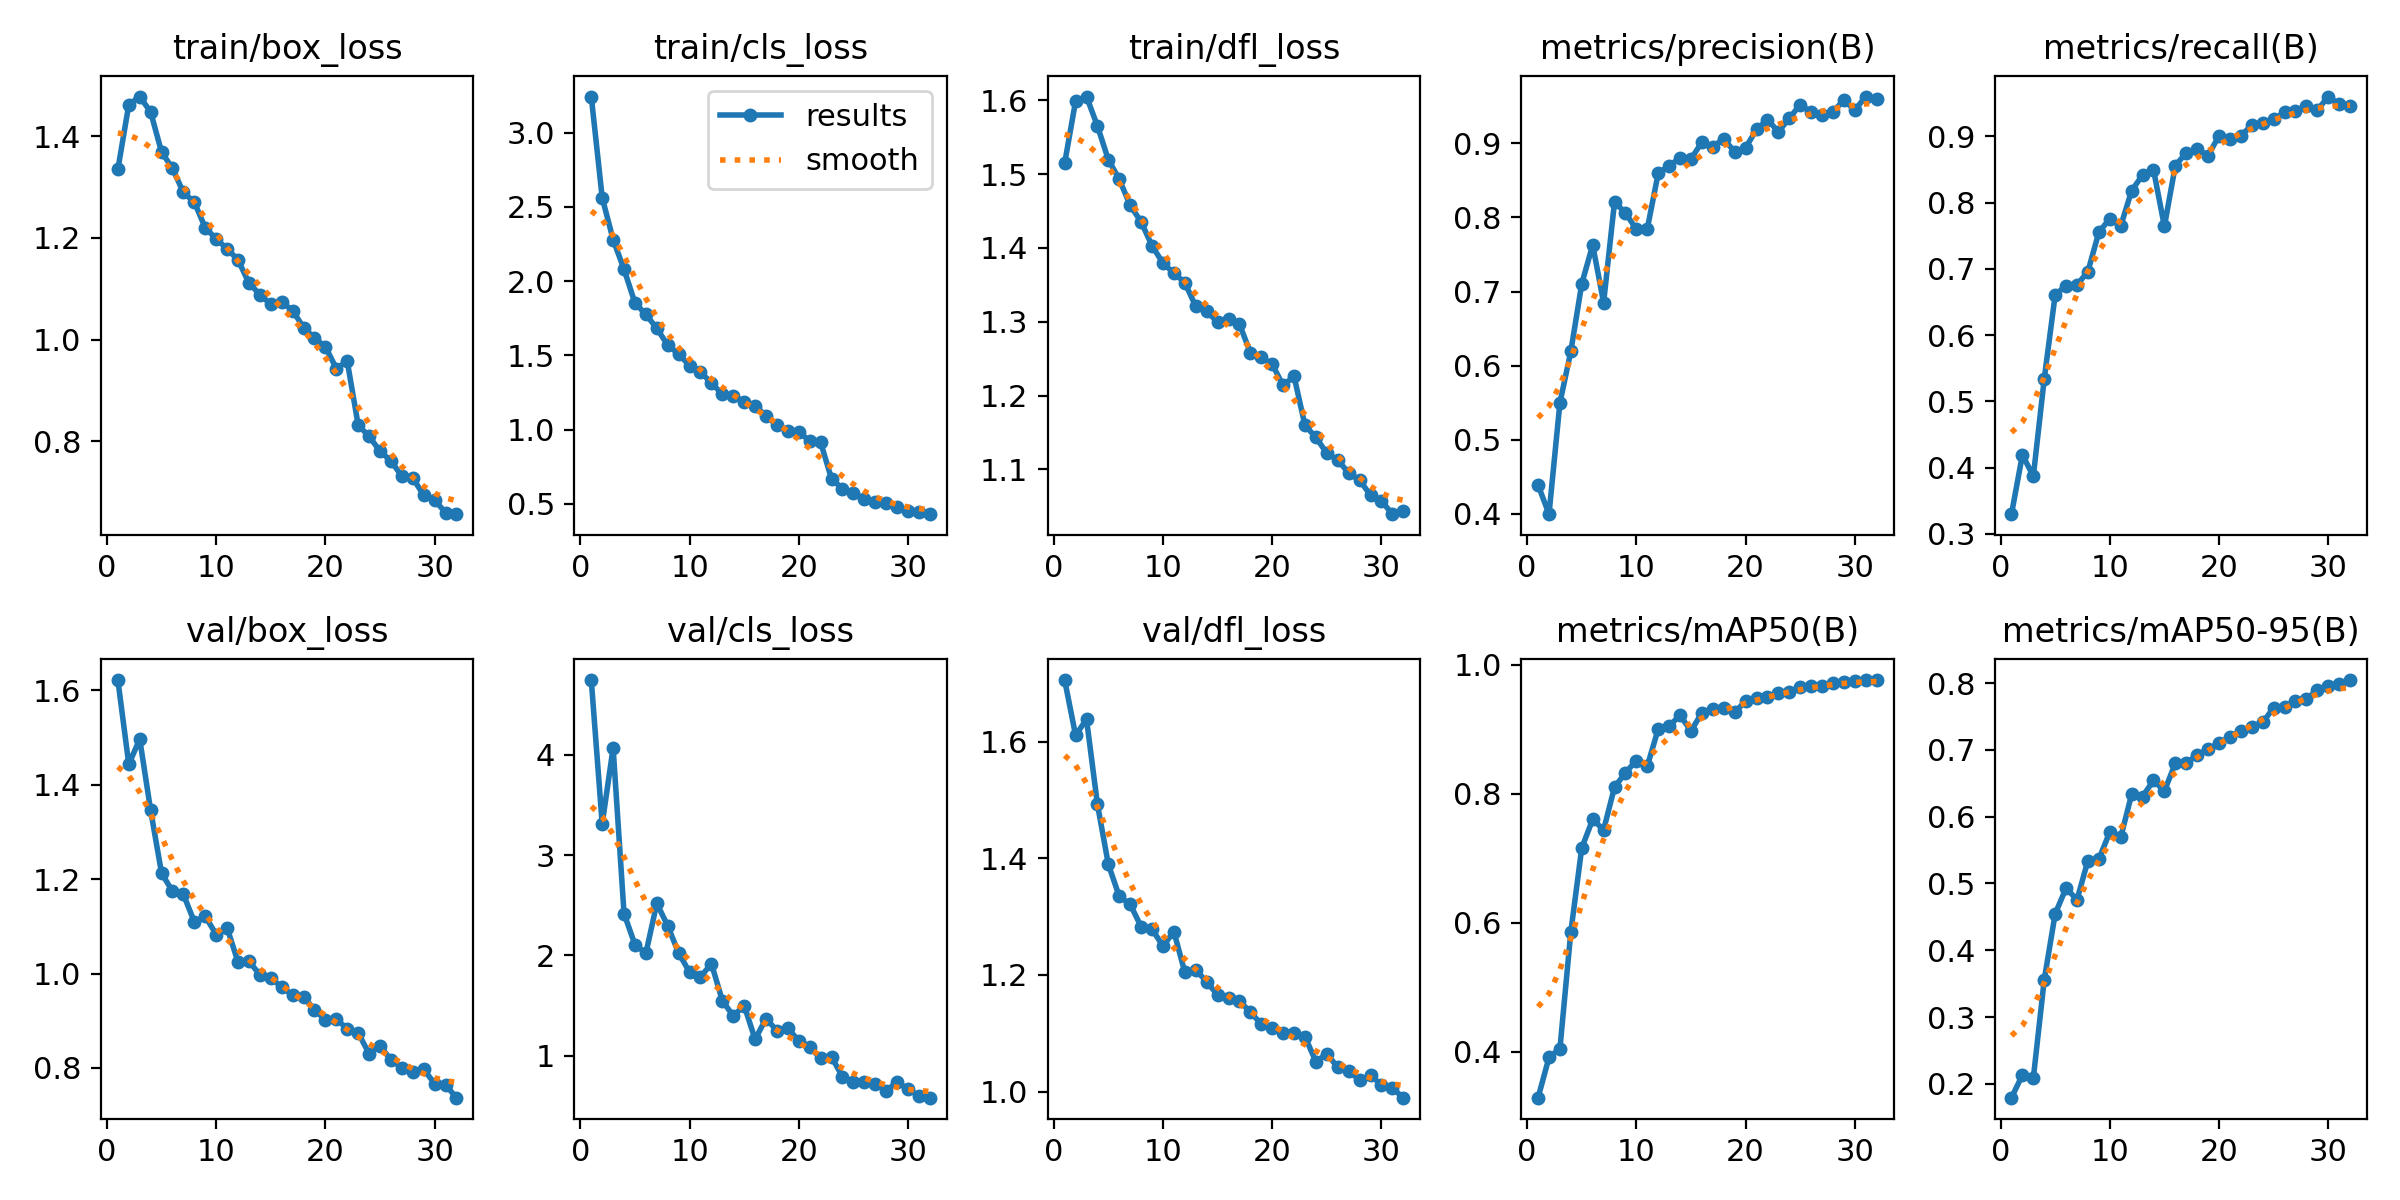
\includegraphics[width=1\textwidth]{./figures/results}
     \caption{Trained Model Metrics}
     \label{fig:red}
\end{figure}
Performance metrics are essential tools for assessing the accuracy and efficiency of object detection models. They provide valuable insights into a model's ability to correctly identify and localize objects within images. Additionally, these metrics help us understand how well the model manages false positives (incorrectly identifying an object that is not there) and false negatives (failing to detect an object that is present). Such insights are indispensable for evaluating the model's overall performance and identifying areas for improvement. In this guide, we will explore the various performance metrics used in the context of $YOLOv8$, discuss their importance, and explain how to interpret them effectively.

Metrics such as $Precision$, $Recall$, and the $F1$ $score$ are commonly used to measure the performance of object detection models. $Precision$ quantifies the accuracy of the positive predictions made by the model, while $Recall$ measures the model's ability to identify all relevant objects in the images. The $F1$ $score$, which is the harmonic mean of $Precision$ and $Recall$, provides a single metric that balances both concerns. Additionally, metrics like Average Precision $(AP)$ and Mean Average Precision $(mAP)$ are particularly significant in object detection. They summarize the model's performance across different thresholds, offering a comprehensive view of its effectiveness.

The Intersection over Union (IoU) metric is another crucial measure. It evaluates the overlap between the predicted bounding boxes and the ground truth bounding boxes. A higher IoU indicates better accuracy in object localization. By examining these metrics, one can gauge the strengths and weaknesses of the model in various scenarios, enabling targeted improvements and optimizations. As we know, in a model development pipeline, the process doesn't stop at training and validating the model. Another crucial step is testing the model we have just trained. Testing the model is essential for evaluating its performance on unseen data, which simulates real-world scenarios and ensures that the model generalizes well beyond the training and validation datasets. Testing serves multiple purposes:

\begin{itemize}
    \item[\textbullet] \textbf{Performance Evaluation}: Testing provides a final assessment of the model's accuracy, precision, recall, and other relevant metrics. This step helps determine if the model meets the desired performance criteria and is ready for deployment.
    \item[\textbullet] \textbf{Generalization Capability}: By testing on unseen data, we can measure how well the model generalizes to new, real-world data. This helps identify any overfitting that may have occurred during training, where the model performs well on training data but poorly on new data.
    \item[\textbullet] \textbf{Robustness Analysis}: Testing allows us to analyze the model's robustness under various conditions. This includes evaluating the model's performance across different lighting conditions, object occlusions, and other challenging scenarios that it might encounter in real-world applications.
    \item[\textbullet] \textbf{Error Analysis}: During testing, we can identify specific cases where the model fails or performs suboptimally. This analysis provides valuable insights into the model's weaknesses and guides further improvements and refinements.
    \item[\textbullet] \textbf{Benchmarking}: Testing provides a standardized way to compare the performance of different models or approaches. By using consistent testing protocols and datasets, we can objectively evaluate the strengths and weaknesses of various models and select the best one for the task at hand.
\end{itemize}

\begin{figure}[H]
     \centering
     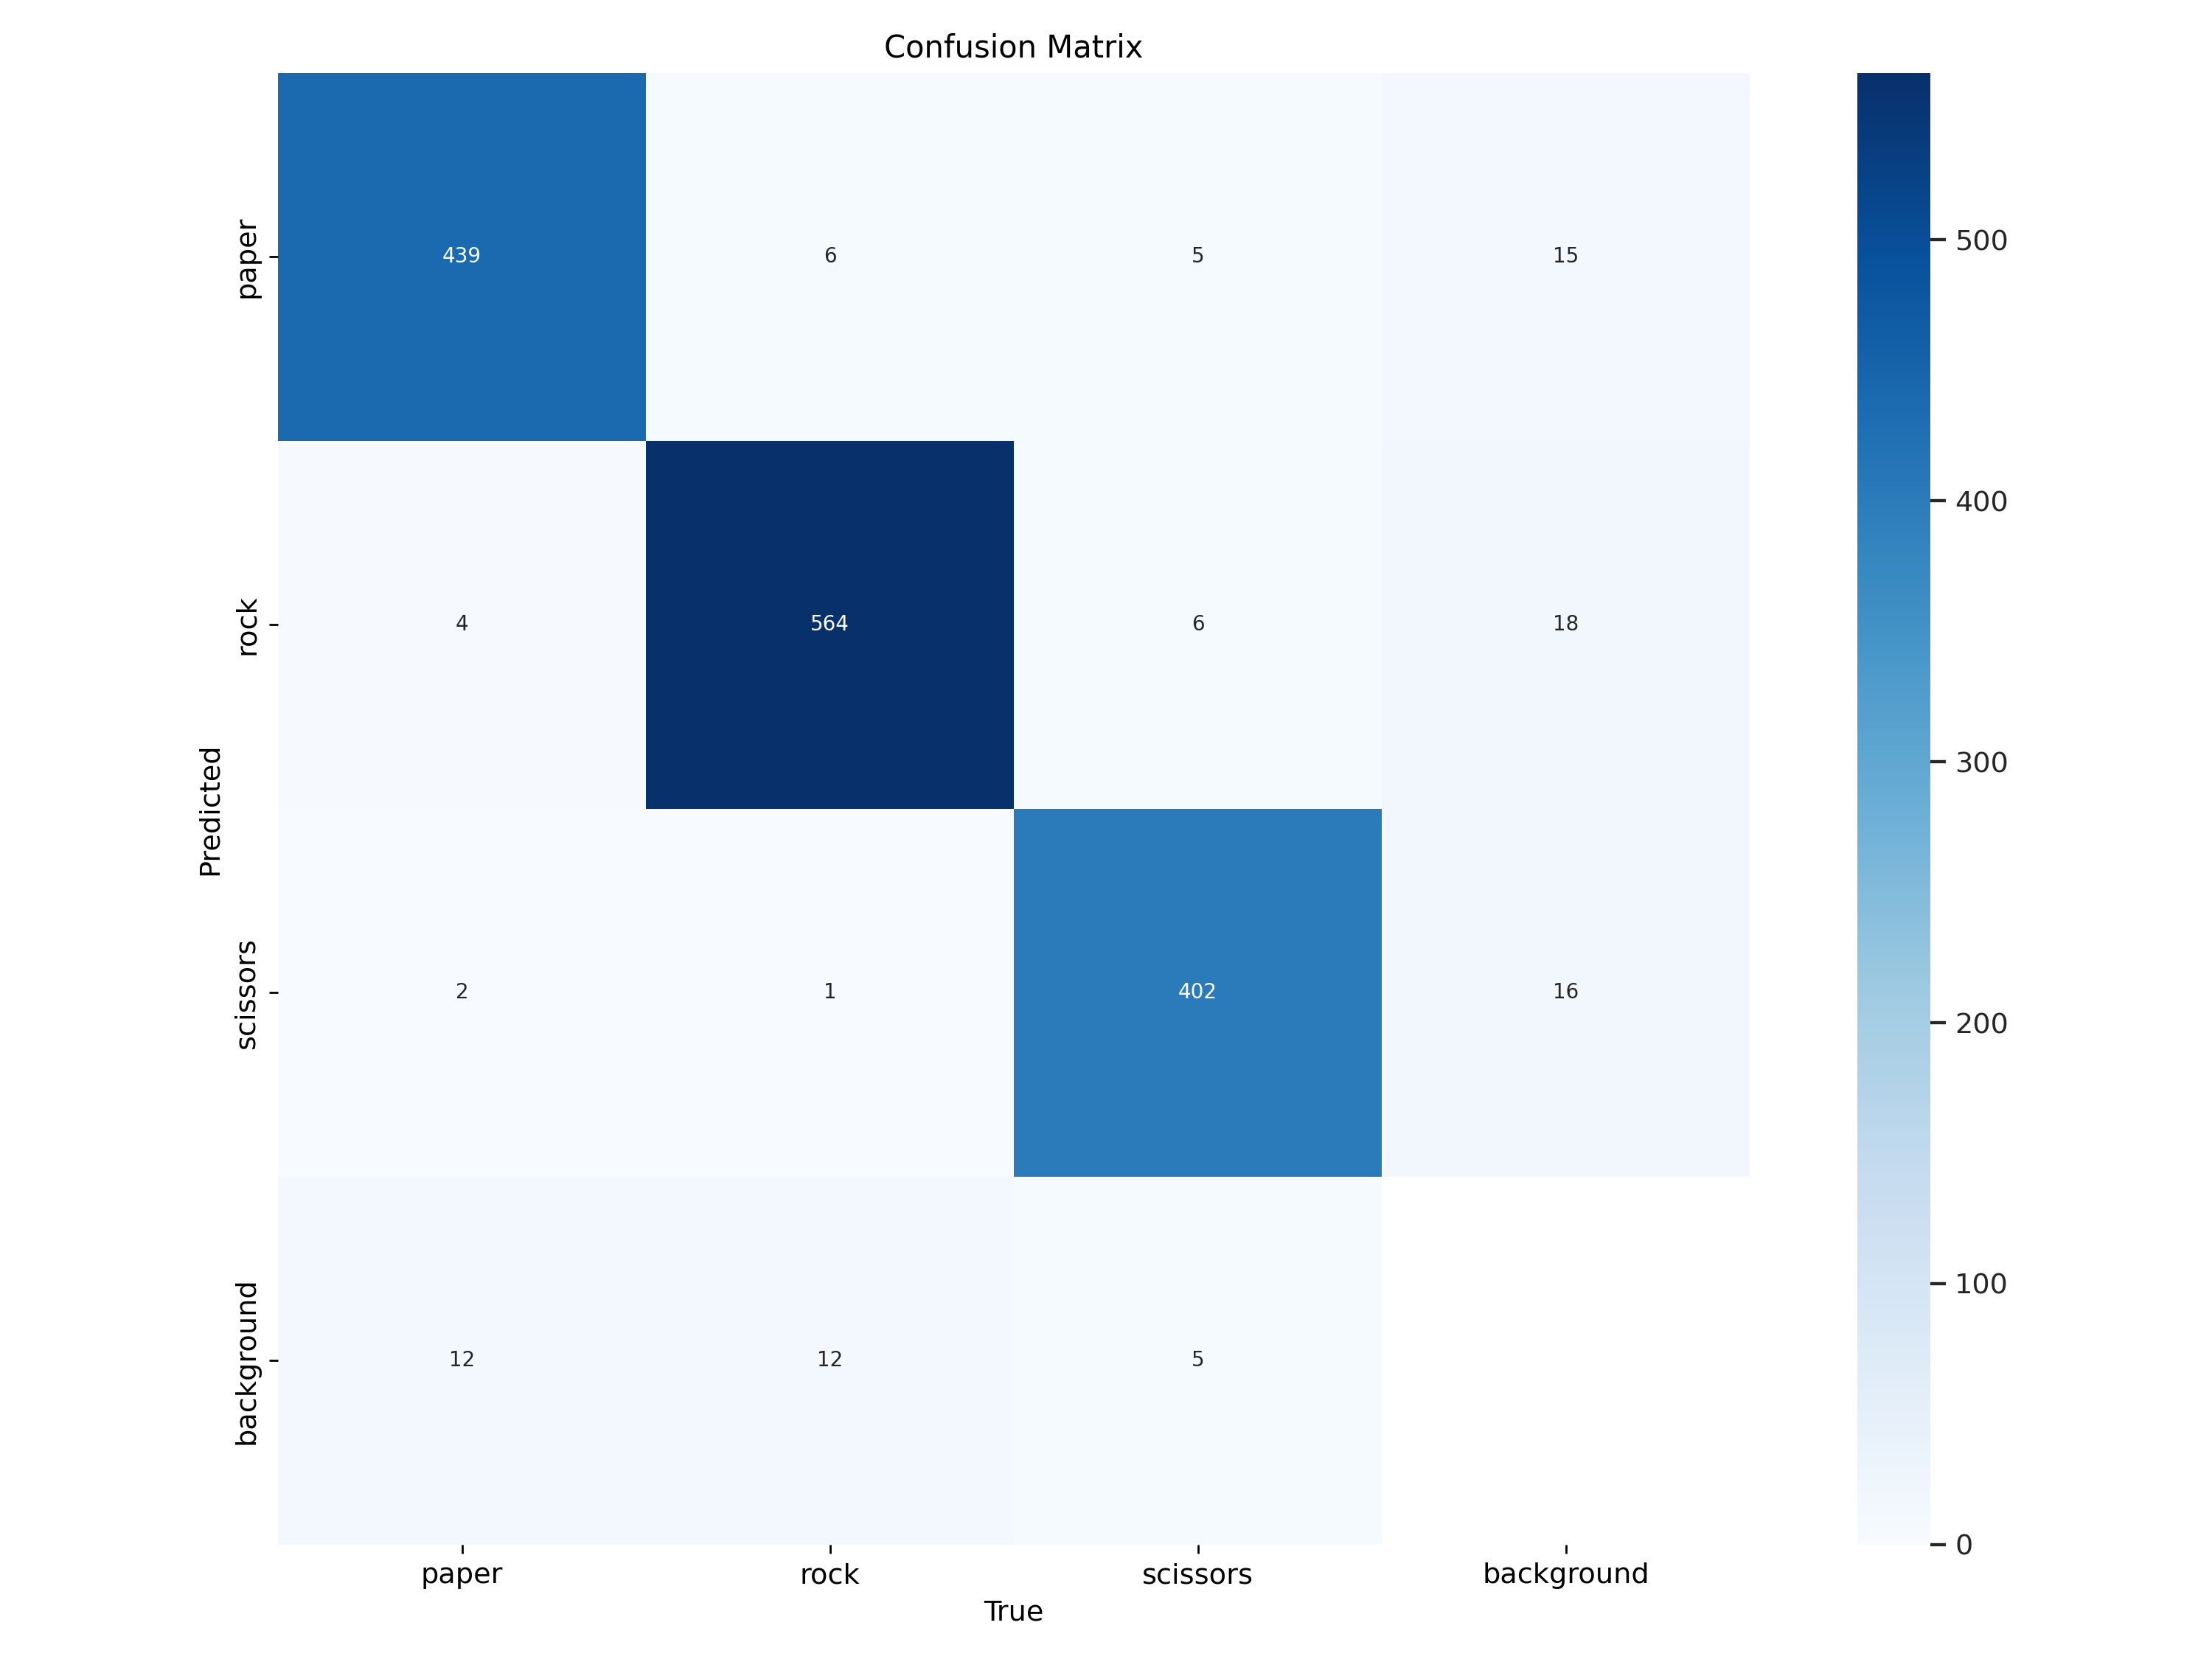
\includegraphics[width=1\textwidth]{./figures/confusion_matrix}
     \caption{Confusion matrix during testing period}
     \label{fig:red}
\end{figure}
\section{Tests to the Model}
We would like to test how well the model can recognize objects using our own prepared images. Here is an example of what the model detects:
\begin{figure}[H]
    \centering
    \begin{minipage}{0.48\textwidth}
        \centering
        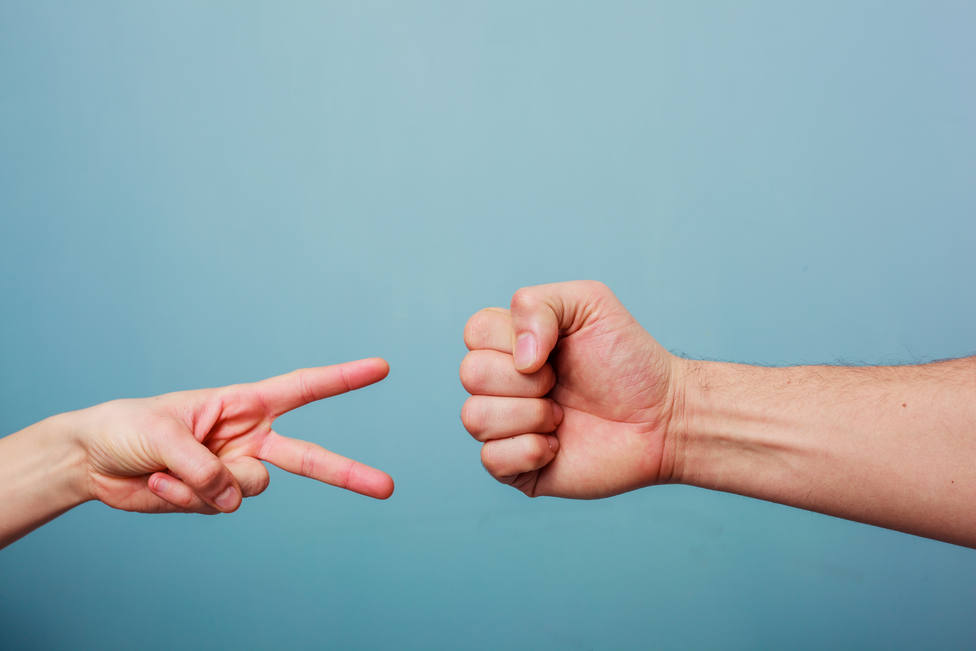
\includegraphics[width=\linewidth]{./figures/try}
        \caption{Test Image}
        \label{fig:example1}
    \end{minipage}\hfill
    %\hspace{0.01\textwidth} % Ajusta este valor según sea necesario para la separación
    \begin{minipage}{0.48\textwidth}
        \centering
        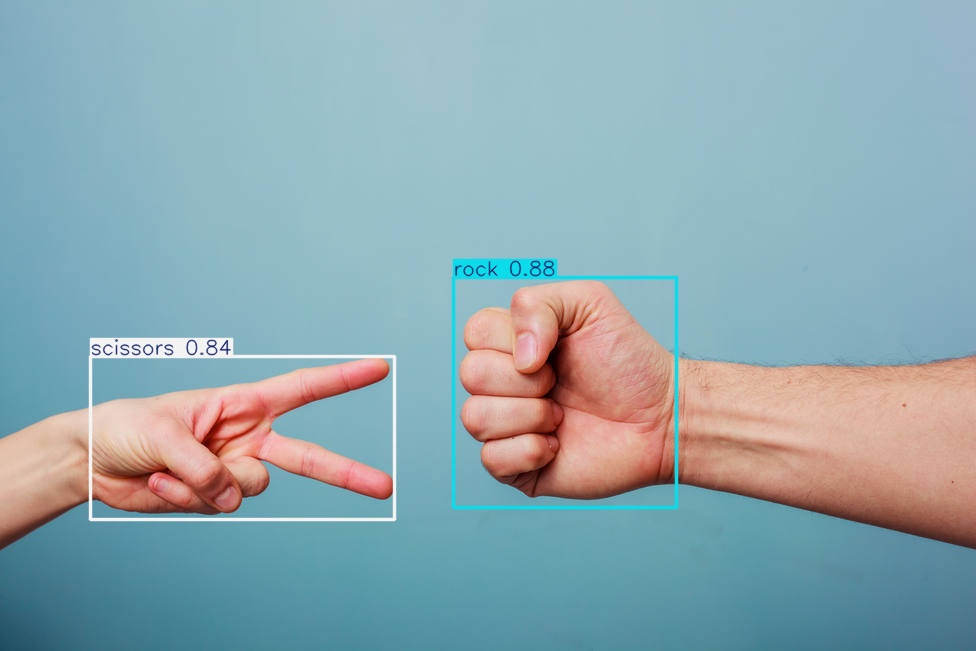
\includegraphics[width=\linewidth]{./figures/res}
        \caption{Test Image Detection}
        \label{fig:example2}
    \end{minipage}
\end{figure}

\end{document}